\subsection{Ellipse parametric equation}

\begin{table}[ht]
	\begin{center}
		\begin{tabular}[top]{ |p{16.0 cm}| }
			\rowcolor{LIGHTCYAN}			
		%%	\hline \multicolumn{1}{|c|}{\textbf{Part 2/5 Ellipse and Skewed-Astroid parametric curves}} \\ [1.0ex]
			
			
		%%	 // ELLIPSE X
		%%	double scaleup = 11.0;
		%%	double k = (2.0 * PI_cpos);
		%%	double x = sin(k*u);
		%%	return (scaleup)*(x);
			
			
			\hline \textbf{No. 3 - Ellipse parametric curve} \\
			\begin{eqnarray}
				x(u) & = & 11\sin(2\pi u) \nonumber \\   
				y(u) & = & 51\cos(2\pi u) \nonumber \\
				 & \in & [0.0, 1.0] \nonumber
			\end{eqnarray}
			
			Closed loop\\
			Overall Single loop, smooth convex curves\\
			Reflection x-axis: symmetrical\\
			Reflection y-axis: symmetrical\\
			\frame{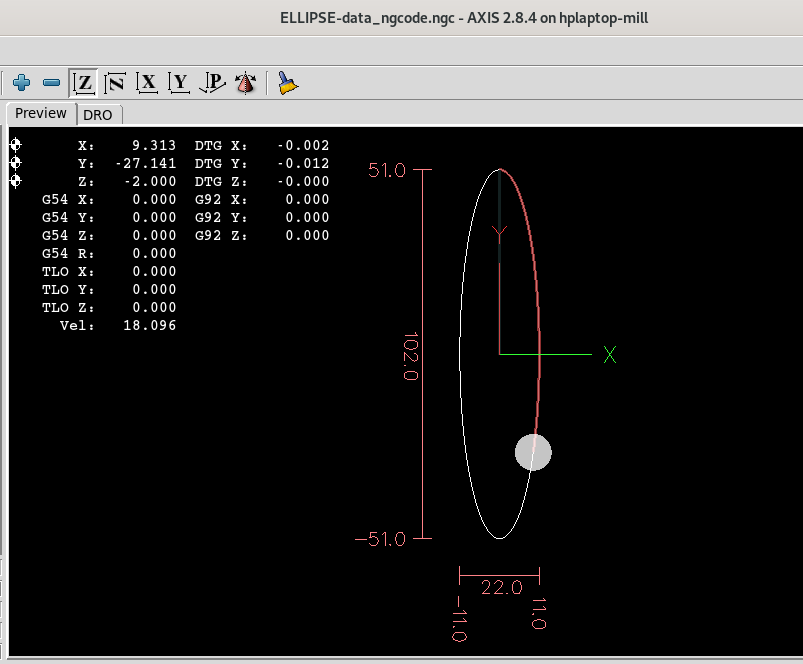
\includegraphics[width=0.51\textwidth]{./07-images/img-Ch5/ELLIPSE-Axis.png}}
			\frame{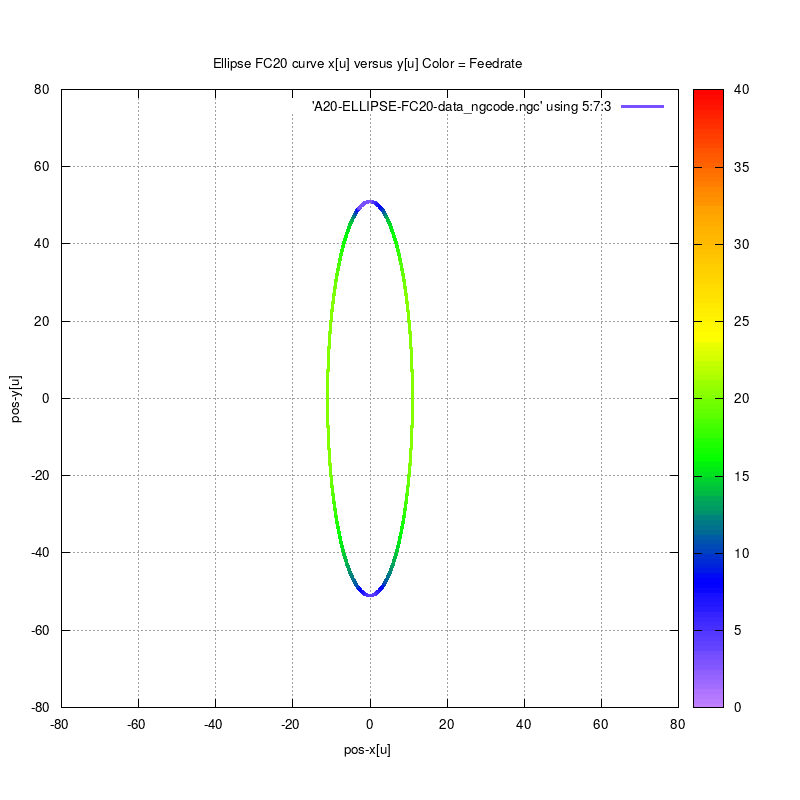
\includegraphics[width=0.42\textwidth]{./07-images/img-Ch5/ELLIPSE-Feedrate.png}}\\
			
			\hline
		\end{tabular}
		\caption{Ellipse equation and dimensions}		
		\label{table:Ellipse equation and dimensions}
	\end{center}
\end{table}  
